\documentclass[UTF8,12pt]{article}
\usepackage{ctex}
\usepackage{indentfirst}
\usepackage{color}
\usepackage{hyperref}
\usepackage{graphicx}
\usepackage{subfigure}
\usepackage{pdfpages}
\usepackage{listings}
\hypersetup{
    hidelinks,
	colorlinks=true,
	allcolors=black,
	pdfstartview=Fit,
	breaklinks=true
}

\definecolor{dkgreen}{rgb}{0,0.6,0}
\definecolor{gray}{rgb}{0.5,0.5,0.5}
\definecolor{mauve}{rgb}{0.58,0,0.82}

\lstset{ %
  language=Octave,                % the language of the code
  basicstyle=\footnotesize,           % the size of the fonts that are used for the code
  numbers=left,                   % where to put the line-numbers
  numberstyle=\tiny\color{gray},  % the style that is used for the line-numbers
  stepnumber=2,                   % the step between two line-numbers. If it's 1, each line 
                                  % will be numbered
  numbersep=5pt,                  % how far the line-numbers are from the code
  backgroundcolor=\color{white},      % choose the background color. You must add \usepackage{color}
  showspaces=false,               % show spaces adding particular underscores
  showstringspaces=false,         % underline spaces within strings
  showtabs=false,                 % show tabs within strings adding particular underscores
  frame=single,                   % adds a frame around the code
  rulecolor=\color{black},        % if not set, the frame-color may be changed on line-breaks within not-black text (e.g. commens (green here))
  tabsize=2,                      % sets default tabsize to 2 spaces
  captionpos=b,                   % sets the caption-position to bottom
  breaklines=true,                % sets automatic line breaking
  breakatwhitespace=false,        % sets if automatic breaks should only happen at whitespace
  title=\lstname,                   % show the filename of files included with \lstinputlisting;
                                  % also try caption instead of title
  keywordstyle=\color{blue},          % keyword style
  commentstyle=\color{dkgreen},       % comment style
  stringstyle=\color{mauve},         % string literal style
  escapeinside={\%*}{*)},            % if you want to add LaTeX within your code
  morekeywords={*,...}               % if you want to add more keywords to the set
}


\setlength{\parindent}{2em}

\begin{document}



\begin{center}
    \tableofcontents
\end{center}
\newpage

\section{实验目标与基本要求}
\subsection{实验目标}
重点结合航空公司客户价值分析的案例介绍K-Means聚类算法在客户价值分析中的应用。此外,介绍基于RFM客户价值分析模型的不足,使用K-Means算法构建航空客户价值分析LRFMC模型,详细的描述数据分析的整个过程。

\subsection{基本要求}
\begin{enumerate}
    \item 了解RFM模型的基本原理。
    \item 掌握K-Means算法的基本原理与使用方法。
    \item 比较不同类别客户的客户价值,制定相应的营销策略。
\end{enumerate}

\section{主要知识点、重点与难点}
\subsection{主要知识点}
\begin{enumerate}
    \item RFM模型的基本原理
    \item K-Means算法的基本原理与使用方法
    \item 比较不同类别客户的客户价值,制定相应的营销策略
\end{enumerate}
    
\subsection{重点}
(1) 航空客户价值分析的步骤和流程。

(2) RFM模型的基本原理。

(3) K-Means算法的基本原理与使用方法。

(4) 比较不同类别客户的客户价值。

\subsection{难点}
(1) RFM模型的基本原理。

(2) KMeans算法的基本原理与使用方法。

\subsection{主要知识点讲解}
\subsubsection{RFM模型}
RFM模型由三个基础指标组成:
\begin{itemize}
    \item 最近一次消费(Recency):客户最近一次消费的时间间隔。间隔越短,表示客户价值越高。
    \item 消费频率(Frequency):客户在最近一段时间内消费的次数。次数越多,表示客户价值越高。
    \item 消费金额(Monetary):客户在最近一段时间内消费的金额。金额越多,表示客户价值越高。
\end{itemize}
在RFM模型里,三个变量的含义都是很具体的。
\begin{figure}[htbp]
    \centering
    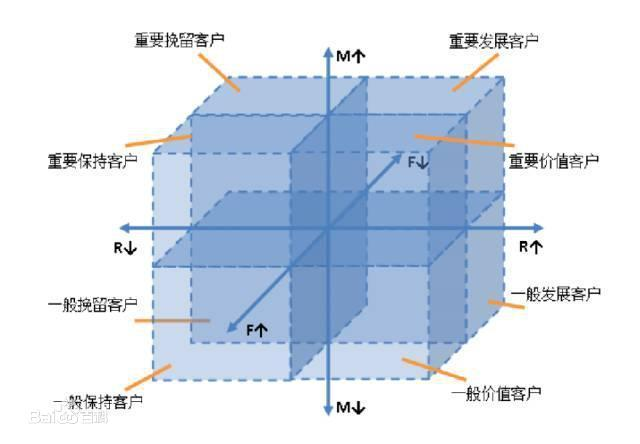
\includegraphics[width=0.6\textwidth]{img/1.png}
    \caption{RFM模型示意图}
\end{figure}

\newpage
但是,RFM模型存在着一个明显的缺陷,那就是没有关注客户的消费周期和消费行为,比如说,作为航空公司,不知道客户是坐头等舱和经济舱,这就催生了LRFMC模型的出现。

\subsubsection{LRFMC模型}
传统的RFM模型它是依据各个属性的平均值进行划分,但是,细分的客户群太多,精准营销的成本太高。因此LRFMC模型将客户聚类为重要保持客户,重要发展客户,重要挽留客户,一般客户,低价值客户,从而针对每种类别的客户制定对应的价格和服务。

一下是LRFMC模型的具体指标:
\begin{figure}[htbp]
    \centering
    
\includegraphics[width=0.8\textwidth]{img/2.png}
    \caption{LRFMC模型指标}
\end{figure}

\subsubsection{K-Means算法}
作为数据挖掘的一个重要研究课题,聚类分析技术越来越受到人们的关注。聚类就是将物理或抽象对象的集合分成多个相似的数据子集,同一个子集内的对象之间具有较高的相似度,而不同子集内的对象差别较大。经过专家学者们的研究,目前聚类算法可以归纳为如下几类:基于划分的方法、基于密度的方法、基于层次的方法、基于模型的方法和高维数据的方法。K-means算法作为一种基于划分的动态聚类算法,它以误差平方和SSE作为聚类准则函数,具有简单有效、收敛速度较快、便于处理大型数据集等优点,从而获得了广泛的应用。

简单总结起来就是:初始化聚类中心、样本点划分、更新聚类中心、样本点划分、更新聚类中心....直至收敛即可。

\begin{figure}[htbp]
    \centering
    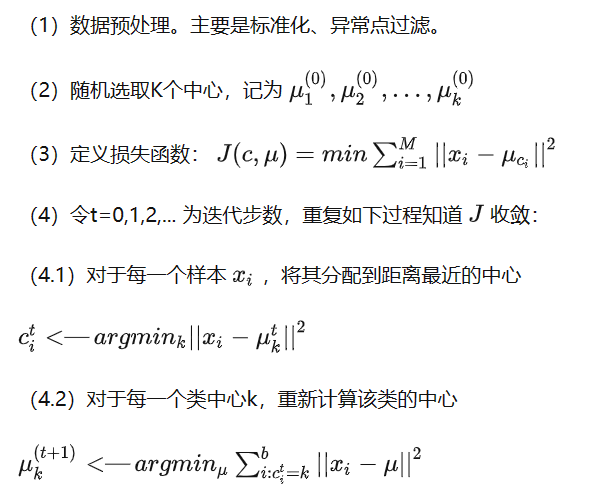
\includegraphics[width=0.7\textwidth]{img/3.png}
    \caption{K-Means算法步骤}
\end{figure}

\section{实验过程设计}
\subsection{实验理论}
(1) 分析航空公司现状。

(2) 认识客户价值分析。

(3) 熟悉航空客户价值分析的步骤与流程。

(4) 处理缺失值与异常值。

(5) 构建爱你航空客户价值分析关键特征。

(6) 标准化LRFMC 5个特征。

(7) 了解K-Means聚类算法。

(8) 分析聚类结果。

(9) 模型应用。

\subsection{实验教学过程}
(1) 处理数据缺失值与异常值。

(2) 构建航空客户价值分析的关键特征。

(3) 标准化LRFMC 5个特征。

(4) 构建K-Means聚类模型。

(5) 评价K-Means聚类模型。

\section{主要实现过程}
\subsection{数据预处理}
\subsubsection{数据清洗}
数据清洗是数据挖掘的第一步,也是最重要的一步。数据清洗的目的是检查数据是否有错误,以及是否有对于分析过程无用的数据。数据清洗的主要任务是填补缺失值和处理异常值。

首先调用describe()函数将air\_data.csv的文件导入,并分别查看数据的缺失值和异常值。函数的输出是两个文件,一个是数据描述.csv,记录各个属性的数据描述;另一个是空值项数量.csv,记录各个属性的空值项数量。

describe()函数的代码如下:
\begin{lstlisting}[title=describe()函数,frame=shadowbox]
    # 查看数据的整体情况和缺失值
    def describe():
        airline_data = pd.read_csv("../data/air_data.csv",
                                   encoding="gb18030")  # 导入航空数据
        explore = airline_data.describe().T
        explore['null'] = len(airline_data) - explore['count']
        explore.to_csv('数据描述.csv')
        df = explore[['max', 'min', 'null']]
        nullData = df[df['null'] > 0]
        nullData = nullData['null']
        nullData.to_csv('空值项数量.csv')
        return airline_data
\end{lstlisting}

运行程序之后,得到两个csv文件,分别是数据描述.csv和空值项数量.csv。数据描述.csv的内容如下:

\begin{figure}[htbp]
    \centering
    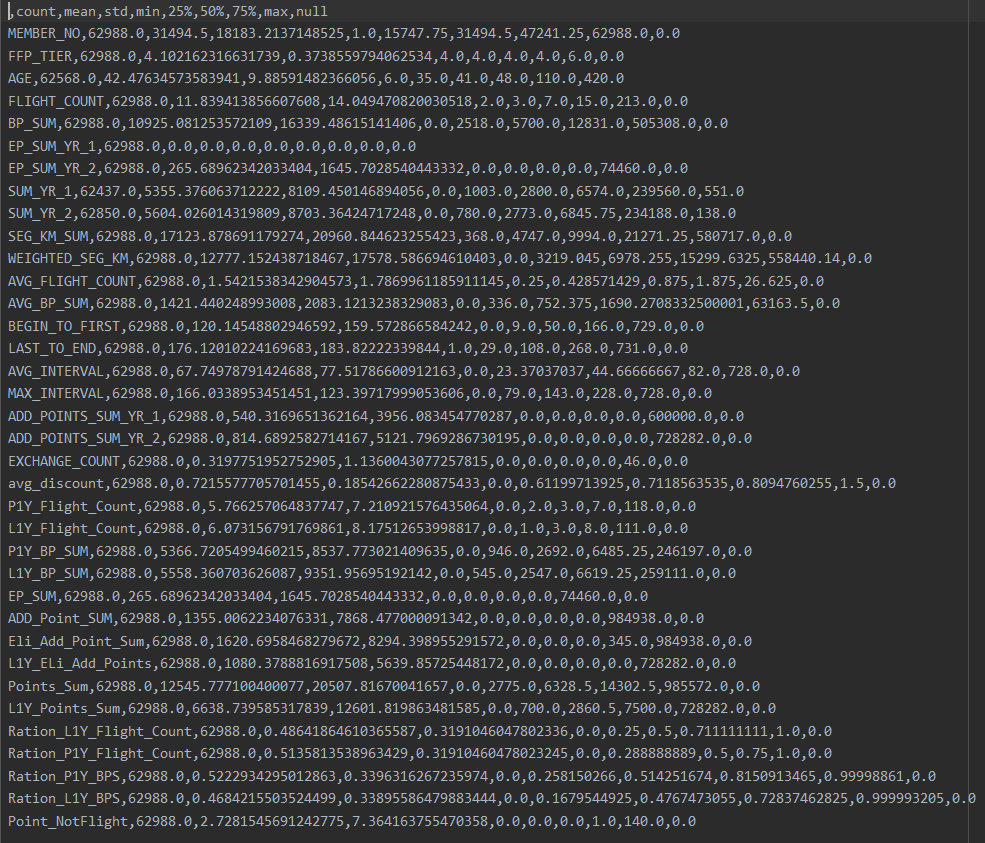
\includegraphics[width=0.8\textwidth]{img/4.png}
    \caption{数据描述.csv}
\end{figure}

空值项数量.csv的内容如下:

\begin{figure}[htbp]
    \centering
    
\includegraphics[width=0.1\textwidth]{img/5.png}
    \caption{空值项数量.csv}
\end{figure}

可以看到其中AGE缺失420条数据,SUM\_YR\_1缺失551条数据,SUM\_YR\_2缺失138条数据。这些缺失值的存在会影响到后续的数据分析,因此需要对缺失值进行处理,本实验中由于样本数量比较庞大,因此删除少量数据不会影响到整体的分析结果,因此采用删除缺失值的方法进行处理。

利用notnull()函数筛选出air\_data.csv中不为空值的行,将SUM\_YR\_1和SUM\_YR\_2中的非空值做与运算,再通过loc()函数筛选出airline\_notnull,实现上述操作的代码如下:

\begin{lstlisting}[title=删除缺失值,frame=shadowbox]
    # 删除缺失值和异常值
    def data_cleaning(airline_data):
        exp1 = airline_data["SUM_YR_1"].notnull()
        exp2 = airline_data["SUM_YR_2"].notnull()
        exp = exp1 & exp2
        print(exp)
        print('exp的形状是:', exp.shape)
        airline_notnull = airline_data.loc[exp, :]
        print('删除缺失记录后数据的形状为:', airline_notnull.shape)
\end{lstlisting}

得到删除缺失值之后数据的结果:

\begin{figure}[htbp]
    \centering
    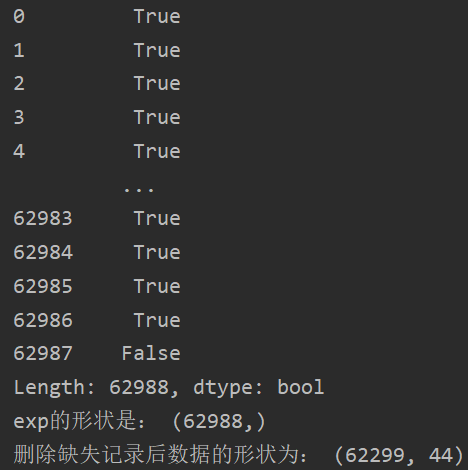
\includegraphics[width=0.3\textwidth]{img/6.png}
    \caption{删除缺失值后的数据}
\end{figure}

得到的删除缺失值后的数据的形状为(62299,44),即删除了缺失值后的数据集中还剩下62299条数据。但是这些数据中仍然存在异常值,因此需要对异常值进行处理。

需要丢弃第一年或者第二年票价为0,平均折扣不为0同时总飞行公里数大于0的记录。在airline\_notnull的基础上进行操作,并将预处理完的数据返回,操作代码如下:

\begin{lstlisting}[title=删除缺失值+处理异常值,frame=shadowbox]
    # 删除缺失值和异常值
    def data_cleaning(airline_data):
        exp1 = airline_data["SUM_YR_1"].notnull()
        exp2 = airline_data["SUM_YR_2"].notnull()
        exp = exp1 & exp2
        # print(exp)
        # print('exp的形状是:', exp.shape)
        airline_notnull = airline_data.loc[exp, :]
        print('删除缺失记录后数据的形状为:', airline_notnull.shape)
    
        # 只保留票价非零的,或者平均折扣率不为0且总飞行公里数大于0的记录。
        index1 = airline_notnull['SUM_YR_1'] != 0
        index2 = airline_notnull['SUM_YR_2'] != 0
        index3 = (airline_notnull['SEG_KM_SUM'] > 0) & \
                 (airline_notnull['avg_discount'] != 0)
        airline = airline_notnull[(index1 | index2) & index3]
        print('删除异常记录后数据的形状为:', airline.shape)
        return airline
\end{lstlisting}

删除缺失值和异常值之后数据的形状为:

\begin{figure}[htbp]
    \centering
    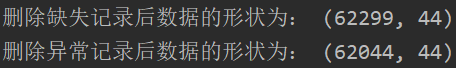
\includegraphics[width=0.3\textwidth]{img/7.png}
    \caption{删除缺失值+处理异常值后的数据}
\end{figure}

\subsubsection{数据筛选}
根据上面的LRFMC模型,只有第一个特征量L是需要进行计算的,通过to\_datetime()函数进行时间间隔的计算,然后强制转换成字符串类型,选取其中的天数,再通过天数获得月份,最后连接上原始数据集,得到最终筛选好的的数据集,代码如下:

\begin{lstlisting}[title=数据筛选,frame=shadowbox]
    # 数据筛选
def data_selection(airline):
    # 选取需求特征
    """
    L: 入会时间
    FLIGHT_COUNT: F 乘机次数
    LAST_TO_END: R 最近消费次数
    avg_discount: C 折扣率
    SEG_KM_SUM: M 飞行里程数
    """
    airline_selection = airline[["FFP_DATE", "LOAD_TIME",
                                 "FLIGHT_COUNT", "LAST_TO_END",
                                 "avg_discount", "SEG_KM_SUM"]]
    L = pd.to_datetime(airline_selection["LOAD_TIME"]) - \
        pd.to_datetime(airline_selection["FFP_DATE"])
    L = L.astype("str").str.split(' ').str[0]
    # 获得会员入会的月数
    L = L.astype("int") / 30
    # 合并特征
    airline_features = pd.concat([L, airline_selection.iloc[:, 2:]], axis=1)
    return airline_features

\end{lstlisting}

构建的LRFMC特征前五的行为如下:

\begin{figure}[htbp]
    \centering
    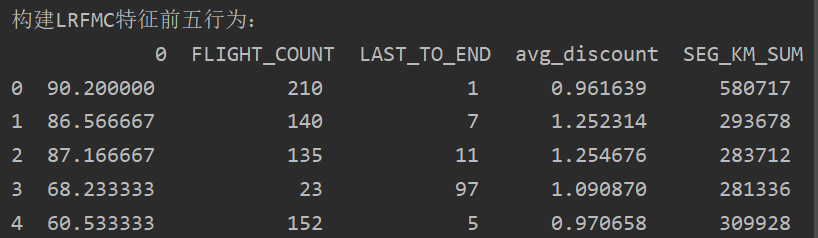
\includegraphics[width=0.8\textwidth]{img/8.png}
    \caption{LRFMC特征前五的行}
\end{figure}

\subsubsection{数据标准化处理}
对完成上述数据处理完之后的数据集进行标准化处理。函数中使用sklearn的StandardScaler对"airline\_features"数据进行标准化,并将结果保存到全局变量"data"中。代码如下:

\begin{lstlisting}[title=数据标准化处理,frame=shadowbox]
    # 数据标准化
    def data_normalization(airline_features):
        global data
        data = StandardScaler().fit_transform(airline_features)
        np.savez('../tmp/airline_scale.npz', data)
        print('标准化后LRFMC五个特征为:\n', data[:5, :])
\end{lstlisting}

标准化后的LRFMC五个特征为:

\begin{figure}[htbp]
    \centering
    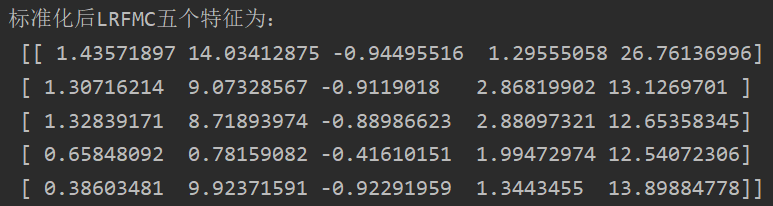
\includegraphics[width=0.8\textwidth]{img/9.png}
    \caption{标准化后的LRFMC五个特征}
\end{figure}

\subsection{数据分析}
\subsubsection{读取数据}
read\_data()函数从保存的文件中加载经过预处理和标准化的航空数据。

\begin{lstlisting}[title=读取数据,frame=shadowbox]
    def read_data():
        airline_scale = np.load('../tmp/airline_scale.npz')['arr_0']
        return airline_scale
\end{lstlisting}

\subsubsection{K-Means聚类分析}
cluster()函数使用scikit-learn中的K-Means算法对航空数据进行K均值聚类。它将聚类中心数(k)设置为5,拟合模型并打印聚类中心和标签。

\begin{lstlisting}[title=K-Means聚类分析,frame=shadowbox]
    # 聚类数据分析
    def cluster(airline_scale):
        k = 5   # 聚类中心数
        kmeans_model = KMeans(n_clusters=k, n_init=4, random_state=666)
        kmeans_model.fit(airline_scale)  # 模型训练
        print('聚类中心:\n', kmeans_model.cluster_centers_)  # 查看聚类中心
        print('类别标签:\n', kmeans_model.labels_)  # 查看样本的类别标签
        # 统计不同类别样本的数目
        r1 = pd.Series(kmeans_model.labels_).value_counts()
        print('最终每个类别的数目为:\n', r1)
        return kmeans_model
\end{lstlisting}

模型训练后,得到的聚类中心、样本类别标签以及每个类别的数量:

\begin{figure}[htbp]
    \centering
    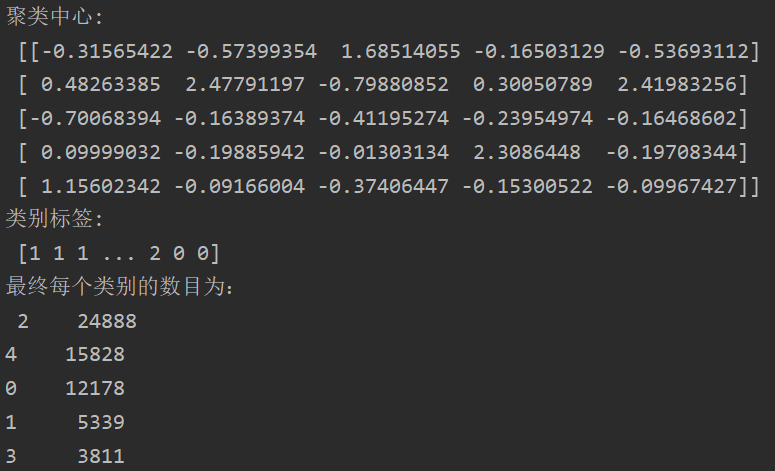
\includegraphics[width=0.8\textwidth]{img/10.png}
    \caption{K-Means聚类分析结果}
\end{figure}

\subsection{聚类模型评价}
\subsubsection{FMI评价法}
Fowlkes–Mallows指数是一种外部评估方法,用于确定两个聚类(通过聚类算法获得的聚类)之间的相似性,也是衡量混淆矩阵的指标。这种相似性度量可以是两个层次聚类之间的相似性,也可以是一个聚类和一个基准分类之间的相似性。FMI的取值范围为[0,1],值越大,聚类结果越好。FMI的计算公式如下:
$$FM=\sqrt{PPV \cdot TPR}=\sqrt{\frac{TP}{TP+FP} \cdot \frac{TP}{TP+FN}}$$

函数使用scikit-learn的fowlkes\_mallows\_score函数,计算不同聚类数(2到6)下的Fowlkes-Mallows指数(FMI)。代码如下:

\begin{lstlisting}[title=FMI评价法,frame=shadowbox]
# FMI评价法
def FMI(airline_scale, kmeans_model):
    for i in range(2, 7):
        kmeans = KMeans(n_clusters=i, random_state=123).fit(airline_scale)
        print(kmeans.labels_)
        print(type(kmeans.labels_))
        score = fowlkes_mallows_score(kmeans_model.labels_, kmeans.labels_)
        print('数据聚%d类FMI评价分值为:%f' % (i, score))
\end{lstlisting}

展示结果如下:

\begin{figure}[htbp]
    \centering
    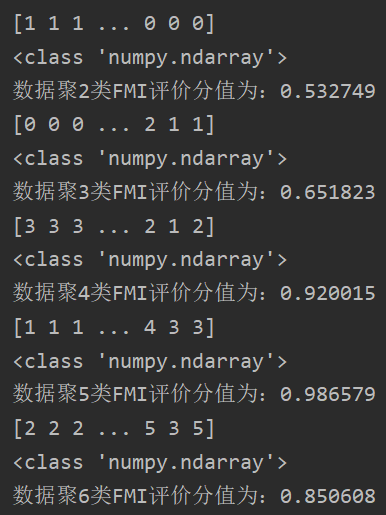
\includegraphics[width=0.6\textwidth]{img/11.png}
    \caption{FMI评价法结果}
\end{figure}


由运算结果得到,数据聚5类的FMI评价分值最高,为0.986579,说明聚类效果最好。
但是由于FMI评价方法需要有明确的标签值,但是本题没有标签(无监督学习),所以使用FMI评价方法计算出来的分数并不具有参考价值。

\subsubsection{轮廓系数(Silhouette Coefficient)评价}
轮廓系数,是用于评价聚类效果好坏的一种指标。可以理解为描述聚类后各个类别的轮廓清晰度的指标。其包含有两种因素——内聚度和分离度。

内聚度可以理解为反映一个样本点与类内元素的紧密程度。

分离度可以理解为反映一个样本点与类外元素的紧密程度。

轮廓系数的公式如下:

$$s(i)=\frac{b(i)-a(i)}{max\{a(i),b(i)\}}$$

其中$a(i)$是样本$i$与同簇其他样本的平均距离,$b(i)$是样本$i$与最近其他簇的平均距离。

$a(i)$的计算公式是:

$$a(i)=\frac{1}{n-1} \sum_{j \neq i}^n distance(i,j)$$

$b(i)$的计算公式与$a(i)$类似,是样本$i$与其他簇的平均距离。只不过需要遍历所有的簇,找到最近的那个簇。

所有样本$S_i$的轮廓系数的均值就是聚类结果的轮廓系数,定义为$S$,是该聚类是否合理、有效的度量。聚类结果的轮廓系数的取值在$[-1,1]$之间,值越大,说明同类样本相距越近、不同样本相距越远,则聚类效果越好;当轮廓系数为负值时,说明聚类结果不合理。

计算轮廓系数的代码如下:

\begin{lstlisting}[title=轮廓系数评价,frame=shadowbox]
    # silhouetteScore相似度评价法
def SS(airline_scale):
    silhouetteScore = []
    for i in range(2, 7):
        kmeans = KMeans(n_clusters=i, random_state=123).fit(airline_scale)
        score = silhouette_score(airline_scale, kmeans.labels_)
        print('航空公司数据聚%d类silhouette评价分值为:%f' % (i, score))
        silhouetteScore.append(score)
    plt.figure(figsize=(10, 6))
    plt.plot(range(2, 7), silhouetteScore, linewidth=1.5, linestyle="-")
    plt.show()
\end{lstlisting}

运行程序之后,得到2到6类的轮廓系数如下:
\begin{figure}[htbp]
    \centering
    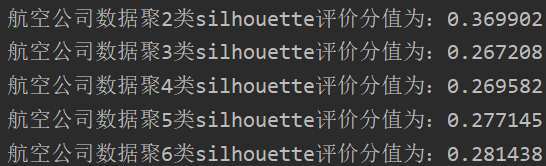
\includegraphics[width=0.6\textwidth]{img/12.png}
    \caption{轮廓系数评价结果}
\end{figure}

在本题中,轮廓系数最大的是2类,此外根据评价结果绘制了轮廓系数与聚类数目的折线图,如下:
\begin{figure}[htbp]
    \centering
    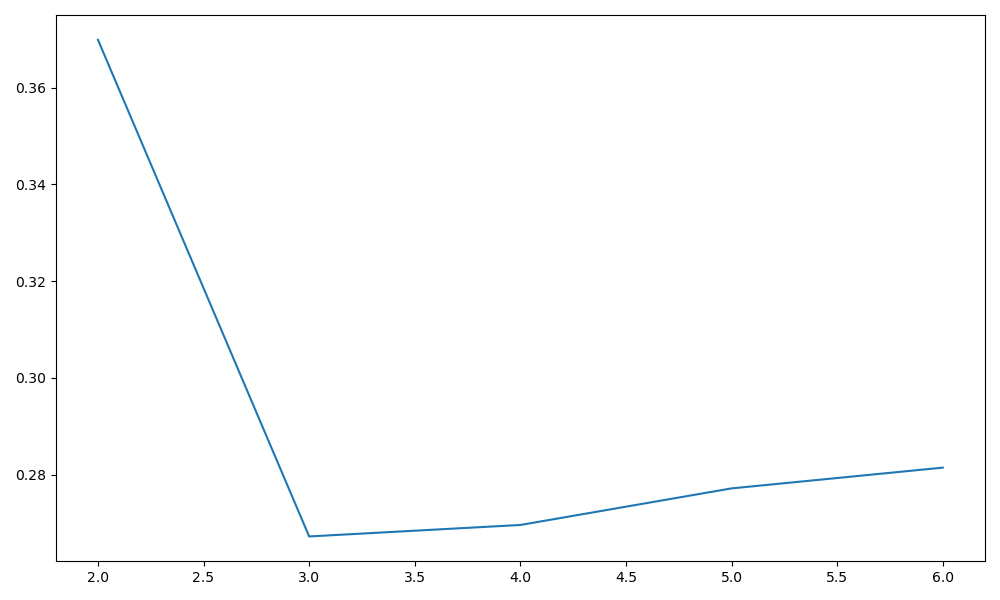
\includegraphics[width=0.4\textwidth]{img/13.png}
    \caption{轮廓系数评价结果}
\end{figure}

\subsubsection{Calinski-Harabasz Index(CH)评价}

Calinski-Harabasz指数的本质是簇间距离与簇内距离的比值,且整体计算过程与方差计算方式类似,所以又将其称之为方差比准则。

将容量为 N 的数据集合 X 聚成 K 类,通过计算类内各点与类中心的距离平方和来度量类内的紧密度(类内距离),各个类中心点与数据集中心点距离平方和来度量数据集的分离度(类间距离)。

CH指标的计算公式为:
$$s=\frac{tr(B_k)}{tr(W_k)} \cdot \frac{N-K}{K-1}$$

其中$tr(B_k)$是类间距离,$tr(W_k)$是类内距离,$N$是样本总数,$K$是类别数。

$B_k$和$W_k$的计算公式如下:
$$B_k=\sum_{i=1}^k n_i \cdot \left \| \mu_i - \mu \right \|^2$$

$$W_k=\sum_{i=1}^k \sum_{x \in C_i} \left \| x - \mu_i \right \|^2$$

Calinski-Harabasz指数的分数越大说明越好(类别内部协方差越小越好,类别之间协方差越大越好)。指数的取值范围为$[0,+\infty)$,但是由于类别数目$K$的限制,所以指数的取值范围为$[0,+\infty)$。

计算CH指数的代码如下:

\begin{lstlisting}[title=CH评价,frame=shadowbox]
    # calinski_harabaz指数评价法
    def CH(airline_scale):
        ch = []
        for i in range(2, 7):
            # 构建并训练模型
            kmeans = KMeans(n_clusters=i, random_state=123).fit(airline_scale)
            score = calinski_harabasz_score(airline_scale, kmeans.labels_)
            print('航空公司数据聚%d类calinski_harabaz指数为:%f' % (i, score))
            ch.append(score)
        plt.figure(figsize=(10, 6))
        plt.plot(range(2, 7), ch, linewidth=1.5, linestyle="-")
        plt.show()
\end{lstlisting}

运行程序之后,得到2到6类的CH指数如下:
\begin{figure}[htbp]
    \centering
    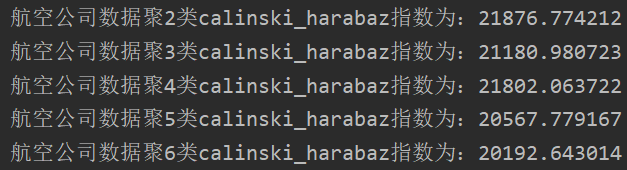
\includegraphics[width=0.6\textwidth]{img/14.png}
    \caption{CH评价结果}
\end{figure}

在本题中,CH指数最大的依然是2类。综合上述的三种评价方法,在聚类数的选择上选择聚类数为3,但是由于LRFMC模型的特殊性,需要将客户划分成五类,所以最终选择聚类数为5。

\subsection{客户价值分析}
\subsubsection{降维图像分析}
TSNE的定位是高维数据可视化。对于聚类来说,输入的特征维数是高维的(大于三维),一般难以直接以原特征对聚类结果进行展示。而TSNE提供了一种有效的数据降维模式,是一种非线性降维算法,可以在2维的空间里展示聚类结果。

在本题中,可以将LRFMC模型的五个维度作为输入,然后将聚类结果进行可视化,代码如下:

\begin{lstlisting}[title=TSNE可视化,frame=shadowbox]
    # 降维图像分析
    def dimensionality_reduction(airline_scale, kmeans_model):
        tsne = TSNE(n_components=2, init='random',
                    random_state=177).fit(airline_scale)
        # init:初始化,可以是PCA或random;随机数种子
        df = pd.DataFrame(tsne.embedding_)  # 将原始数据转换为DataFrame
        print(df)
        df['labels'] = kmeans_model.labels_  # 将聚类结果存储进df数据表
        print(df['labels'])
    
        # 提取不同标签的数据
        df1 = df[df['labels'] == 0]
        df2 = df[df['labels'] == 1]
        df3 = df[df['labels'] == 2]
        df4 = df[df['labels'] == 3]
        df5 = df[df['labels'] == 4]
    
        #  绘制图形
        fig = plt.figure(figsize=(9, 6))  # 设定空白画布,并制定大小
        # 用不同的颜色表示不同数据
        plt.plot(df2[0], df2[1], 'r*')
        plt.plot(df3[0], df3[1], 'gD')
        plt.plot(df4[0], df4[1], 'kD')
        plt.plot(df5[0], df5[1], 'lD')
        plt.savefig('../tmp/聚类结果.png')
        plt.show()  # 显示图片
\end{lstlisting}

\newpage

运行程序之后,得到的降维图像如下:

\begin{figure}[htbp]
    \centering
    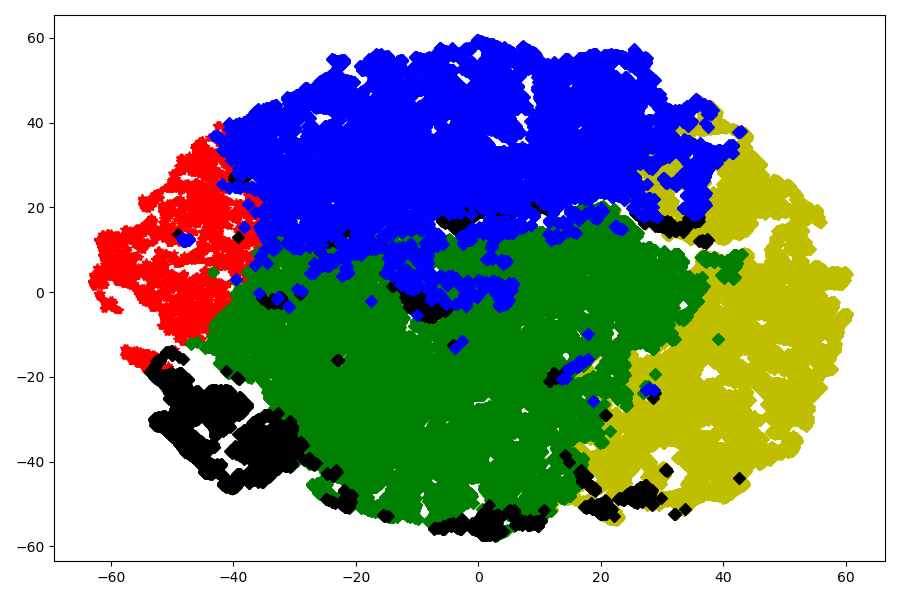
\includegraphics[width=0.8\textwidth]{img/15.png}
    \caption{降维图像}
\end{figure}

从图中可以看出,不同类别的客户被分布在不同的区域,说明聚类结果是比较合理的。

\subsubsection{雷达图分析}
雷达图是一种用于显示多变量数据的图表,它通常以两维的形式绘制,其中每个变量以轴从图表的中心点开始延伸。在本题中,可以将LRFMC模型的五个维度作为输入,然后将聚类结果进行可视化,通过雷达图对客户的价值进行分析代码如下:

\begin{lstlisting}[title=雷达图分析,frame=shadowbox]
    # 画雷达图
    def draw(kmeans_model=None):
        datafile = '标准数据.csv'
        data = pd.read_csv(datafile)
        r2 = pd.DataFrame(kmeans_model.cluster_centers_)  # 聚类的中心数学数值
        print(r2)
        r3 = pd.Series(['客户群1', '客户群2', '客户群3', '客户群4', '客户群5', ])
        labels = np.array(['L', 'R', 'F', 'M', 'C'])  # 标签
        dataLength = 5  # 数据个数
        r4 = r2.T
        print(data.columns)
        r4.columns = list(data.columns)
        fig = plt.figure()
        y = []
        for x in list(data.columns):
            dt = r4[x]
            dt = np.concatenate((dt, [dt[0]]))
            y.append(dt)
        ax = fig.add_subplot(111, polar=True)
        angles = np.linspace(0, 2 * np.pi, dataLength, endpoint=False)
        angles = np.concatenate((angles, [angles[0]]))
        labels = np.concatenate((labels, [labels[0]]))
        ax.plot(angles, y[0], 'b-', linewidth=2)
        ax.plot(angles, y[1], 'r-', linewidth=2)
        ax.plot(angles, y[2], 'g-', linewidth=2)
        ax.plot(angles, y[3], 'y-', linewidth=2)
        ax.plot(angles, y[4], 'm-', linewidth=2)
        plt.rcParams['font.sans-serif'] = ['SimHei']
        plt.rcParams['axes.unicode_minus'] = False  # 用来正常显示负号
        ax.legend(r3, loc=1)
        ax.set_thetagrids(angles * 180 / np.pi, labels, fontproperties="SimHei")
        ax.set_title("用户价值分析雷达图", va='bottom', fontproperties="SimHei")
        ax.grid(True)
        plt.show()
\end{lstlisting}

\newpage

得到的雷达图如下:

\begin{figure}[htbp]
    \centering
    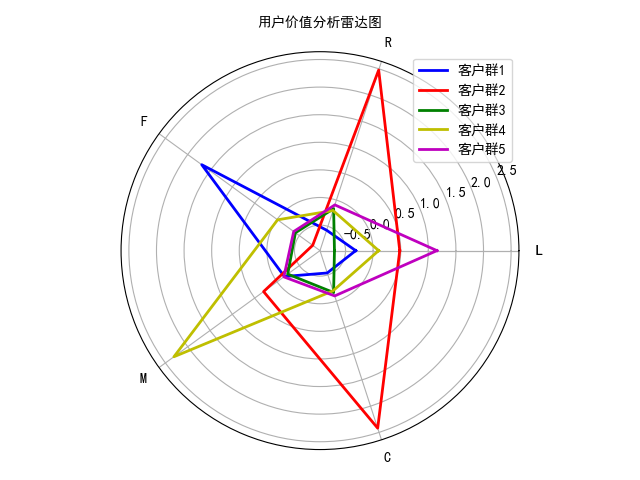
\includegraphics[width=0.8\textwidth]{img/16.png}
    \caption{雷达图}
\end{figure}

通过对雷达图的分析可以得知:

\begin{itemize}
    \item 客户群1:L值较低,R值较低,F值较高,M值较低,C值较低,这类客户经常买票,且比较活跃(上次购票时间较近),但是消费金额较低,这类客户是重要发展客户,应该尽量提高这类客户的消费金额。
    \item 客户群2:L值较高,R值较高,F值较低,M值较低,C值较高,这类客户是老用户,最近消费较少,但是消费金额较高,这类客户是重要挽留客户,应该尽量提高这类客户的忠诚度。
    \item 客户群3:L值较低,R值较低,F值较低,M值较低,C值较低,这类客户是低价值客户,应该尽量避免这类客户流失。
    \item 客户群4:L值较低,R值较低,F值较低,M值较高,C值较低,这类客户是老用户,最近消费多,总飞行里程数高,折扣高,是重要保持客户,应该优先将资源投入到这类客户中。
    \item 客户群5:L值较低,R值较低,F值较低,M值较低,C值较高,这类客户元老级用户,但是享受折扣、频率和里程数都比较低,是一般用户,不在重要维持范围内。
\end{itemize}

重要发展客户、重要保持客户、重要挽留客户分别可以归入航空公司客户生命周期管理的发展期、成熟期和衰退期,而低价值客户和一般用户则可以归入航空公司客户生命周期管理的成长期。

关于五个类别的客户数量如下图

\begin{figure}[htbp]
    \centering
    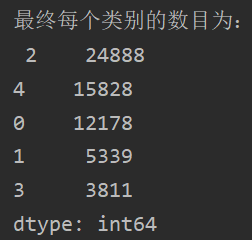
\includegraphics[width=0.6\textwidth]{img/17.png}
    \caption{客户数量}
\end{figure}

可以看出,目前类别2、4、0的客户数量较多,对应的是处于发展期的用户,说明公司正在处于上升期。

\section{总结}
本次实验是对航空公司的客户进行分析,在分析过程中,学习到了LRFMC模型的构建方法,以及如何使用K-Means算法对客户进行聚类,最后通过雷达图对客户进行分析,得到了客户的价值分析结果。

本次实验加强了我对数据挖掘的理解,对于数据挖掘的流程有了更深的认识,同时也加强了我对Python的使用,对于Python的数据分析库有了更深的认识。

当然,在今后的学习中,我还需要继续加强对数据挖掘的理解,同时也需要加强对Python的学习,提高自己的编程能力。

\section{附录}

\subsection{DataPretreatment\.py}

\begin{lstlisting}[title=DataPretreatment\.py,frame=shadowbox]
    import pandas as pd
import numpy as np
from matplotlib import pyplot as plt
from sklearn.manifold import TSNE
from sklearn.preprocessing import StandardScaler


data = []


# 查看数据的整体情况和缺失值
def describe():
    airline_data = pd.read_csv("../data/air_data.csv",
                               encoding="gb18030")  # 导入航空数据
    explore = airline_data.describe().T
    explore['null'] = len(airline_data) - explore['count']
    explore.to_csv('数据描述.csv')
    df = explore[['max', 'min', 'null']]
    nullData = df[df['null'] > 0]
    nullData = nullData['null']
    nullData.to_csv('空值项数量.csv')
    return airline_data


# 删除缺失值和异常值
def data_cleaning(airline_data):
    exp1 = airline_data["SUM_YR_1"].notnull()
    exp2 = airline_data["SUM_YR_2"].notnull()
    exp = exp1 & exp2
    # print(exp)
    # print('exp的形状是:', exp.shape)
    airline_notnull = airline_data.loc[exp, :]
    print('删除缺失记录后数据的形状为:', airline_notnull.shape)

    # 只保留票价非零的,或者平均折扣率不为0且总飞行公里数大于0的记录。
    index1 = airline_notnull['SUM_YR_1'] != 0
    index2 = airline_notnull['SUM_YR_2'] != 0
    index3 = (airline_notnull['SEG_KM_SUM'] > 0) & \
             (airline_notnull['avg_discount'] != 0)
    airline = airline_notnull[(index1 | index2) & index3]
    print('删除异常记录后数据的形状为:', airline.shape)
    return airline


# 数据筛选
def data_selection(airline):
    # 选取需求特征
    """
    L: 入会时间
    FLIGHT_COUNT: F 乘机次数
    LAST_TO_END: R 最近消费次数
    avg_discount: C 折扣率
    SEG_KM_SUM: M 飞行里程数
    """
    airline_selection = airline[["FFP_DATE", "LOAD_TIME",
                                 "FLIGHT_COUNT", "LAST_TO_END",
                                 "avg_discount", "SEG_KM_SUM"]]
    L = pd.to_datetime(airline_selection["LOAD_TIME"]) - \
        pd.to_datetime(airline_selection["FFP_DATE"])
    L = L.astype("str").str.split(' ').str[0]
    # 获得会员入会的月数
    L = L.astype("int") / 30
    # 合并特征
    airline_features = pd.concat([L, airline_selection.iloc[:, 2:]], axis=1)
    print('构建LRFMC特征前五行为:\n',airline_features.head())
    return airline_features


# 数据标准化
def data_normalization(airline_features):
    global data
    data = StandardScaler().fit_transform(airline_features)
    np.savez('../tmp/airline_scale.npz', data)
    print('标准化后LRFMC五个特征为:\n', data[:5, :])


def main():
    airline_data = describe()
    airline = data_cleaning(airline_data)
    airline_features = data_selection(airline)
    data_normalization(airline_features)


if __name__ == '__main__':
    main()

\end{lstlisting}

\subsection{DataAnalysis\.py}

\begin{lstlisting}[title=DataAnalysis\.py,frame=shadowbox]
    import numpy as np
import pandas as pd
from matplotlib import pyplot as plt
from sklearn.cluster import KMeans
from sklearn.manifold import TSNE
from sklearn.metrics import fowlkes_mallows_score, silhouette_score, calinski_harabasz_score


# 读入数据
from sklearn.model_selection import train_test_split
from sklearn.preprocessing import StandardScaler
from sklearn.svm import SVC


def read_data():
    airline_scale = np.load('../tmp/airline_scale.npz')['arr_0']
    return airline_scale


# 聚类数据分析
def cluster(airline_scale):
    k = 5   # 聚类中心数
    kmeans_model = KMeans(n_clusters=k, n_init=4, random_state=666)
    kmeans_model.fit(airline_scale)  # 模型训练
    print('聚类中心:\n', kmeans_model.cluster_centers_)  # 查看聚类中心
    print('类别标签:\n', kmeans_model.labels_)  # 查看样本的类别标签
    # 统计不同类别样本的数目
    r1 = pd.Series(kmeans_model.labels_).value_counts()
    print('最终每个类别的数目为:\n', r1)
    return kmeans_model


# FMI评价法
def FMI(airline_scale, kmeans_model):
    for i in range(2, 7):
        kmeans = KMeans(n_clusters=i, random_state=123).fit(airline_scale)
        print(kmeans.labels_)
        print(type(kmeans.labels_))
        score = fowlkes_mallows_score(kmeans_model.labels_, kmeans.labels_)
        print('数据聚%d类FMI评价分值为:%f' % (i, score))


# silhouetteScore相似度评价法
def SS(airline_scale):
    silhouetteScore = []
    for i in range(2, 7):
        kmeans = KMeans(n_clusters=i, random_state=123).fit(airline_scale)
        score = silhouette_score(airline_scale, kmeans.labels_)
        print('航空公司数据聚%d类silhouette评价分值为:%f' % (i, score))
        silhouetteScore.append(score)
    plt.figure(figsize=(10, 6))
    plt.plot(range(2, 7), silhouetteScore, linewidth=1.5, linestyle="-")
    plt.show()


# calinski_harabaz指数评价法
def CH(airline_scale):
    ch = []
    for i in range(2, 7):
        # 构建并训练模型
        kmeans = KMeans(n_clusters=i, random_state=123).fit(airline_scale)
        score = calinski_harabasz_score(airline_scale, kmeans.labels_)
        print('航空公司数据聚%d类calinski_harabaz指数为:%f' % (i, score))
        ch.append(score)
    plt.figure(figsize=(10, 6))
    plt.plot(range(2, 7), ch, linewidth=1.5, linestyle="-")
    plt.show()


# 用支持向量机预测数据
def SVC_prediction(airline_scale, kmeans_model):
    # 划分测试集和训练集
    airline_data_train, airline_data_test, airline_target_train, airline_target_test = \
        train_test_split(airline_scale, kmeans_model.labels_, test_size=0.2, random_state=666)

    # 数据标准化
    stdScaler = StandardScaler().fit(airline_data_train)
    airline_trainStd = stdScaler.transform(airline_data_train)
    airline_testStd = stdScaler.transform(airline_data_test)

    svm = SVC().fit(airline_trainStd, airline_target_train)
    print('建立的SVM模型为:\n', svm)

    #  预测训练集结果
    airline_target_pred = svm.predict(airline_testStd)
    print('预测前20个结果为:\n', airline_target_pred[:20])


# 画雷达图
def draw(kmeans_model=None):
    datafile = '标准数据.csv'
    data = pd.read_csv(datafile)
    r2 = pd.DataFrame(kmeans_model.cluster_centers_)  # 聚类的中心数学数值
    print(r2)
    r3 = pd.Series(['客户群1', '客户群2', '客户群3', '客户群4', '客户群5', ])
    labels = np.array(['L', 'R', 'F', 'M', 'C'])  # 标签
    dataLength = 5  # 数据个数
    r4 = r2.T
    print(data.columns)
    r4.columns = list(data.columns)
    fig = plt.figure()
    y = []
    for x in list(data.columns):
        dt = r4[x]
        dt = np.concatenate((dt, [dt[0]]))
        y.append(dt)
    ax = fig.add_subplot(111, polar=True)
    angles = np.linspace(0, 2 * np.pi, dataLength, endpoint=False)
    angles = np.concatenate((angles, [angles[0]]))
    labels = np.concatenate((labels, [labels[0]]))
    ax.plot(angles, y[0], 'b-', linewidth=2)
    ax.plot(angles, y[1], 'r-', linewidth=2)
    ax.plot(angles, y[2], 'g-', linewidth=2)
    ax.plot(angles, y[3], 'y-', linewidth=2)
    ax.plot(angles, y[4], 'm-', linewidth=2)
    plt.rcParams['font.sans-serif'] = ['SimHei']
    plt.rcParams['axes.unicode_minus'] = False  # 用来正常显示负号
    ax.legend(r3, loc=1)
    ax.set_thetagrids(angles * 180 / np.pi, labels, fontproperties="SimHei")
    ax.set_title("用户价值分析雷达图", va='bottom', fontproperties="SimHei")
    ax.grid(True)
    plt.show()


# 降维图像分析
def dimensionality_reduction(airline_scale, kmeans_model):
    tsne = TSNE(n_components=2, init='random',
                random_state=177).fit(airline_scale)
    # init:初始化,可以是PCA或random;随机数种子
    df = pd.DataFrame(tsne.embedding_)  # 将原始数据转换为DataFrame
    print(df)
    df['labels'] = kmeans_model.labels_  # 将聚类结果存储进df数据表
    print(df['labels'])

    # 提取不同标签的数据
    df1 = df[df['labels'] == 0]
    df2 = df[df['labels'] == 1]
    df3 = df[df['labels'] == 2]
    df4 = df[df['labels'] == 3]
    df5 = df[df['labels'] == 4]

    #  绘制图形
    fig = plt.figure(figsize=(9, 6))  # 设定空白画布,并制定大小
    # 用不同的颜色表示不同数据
    plt.plot(df2[0], df2[1], 'r*')
    plt.plot(df3[0], df3[1], 'gD')
    plt.plot(df4[0], df4[1], 'kD')
    plt.plot(df5[0], df5[1], 'bD')
    plt.savefig('../tmp/聚类结果.png')
    plt.show()  # 显示图片


def main():
    airline_scale = read_data()
    kmeans_model = cluster(airline_scale)
    # FMI(airline_scale, kmeans_model)
    # SS(airline_scale)
    # CH(airline_scale)
    # SVC_prediction(airline_scale, kmeans_model)
    # dimensionality_reduction(airline_scale, kmeans_model)
    draw(kmeans_model)


if __name__ == '__main__':
    main()

\end{lstlisting}



\end{document}